%!TEX root = ../thesis.tex
%*******************************************************************************
%****************************** Fourth Chapter *********************************
%*******************************************************************************

\chapter{Colocalisation of immune infiltrates and spatial statistics of immune cell-tumour-stroma interaction}

\ifpdf
    \graphicspath{{Chapter4/Figs/Raster/}{Chapter4/Figs/PDF/}{Chapter4/Figs/}}
\else
    \graphicspath{{Chapter4/Figs/Vector/}{Chapter4/Figs/}}
\fi


\section[Introduction]{Introduction}

As mentioned in the introduction, some methods of immune analysis are capable of measuring many more markers on a single section than standard IHC and IF. IMC is one of the best of such methods, allowing for measuring more than 20 markers on a single tissue section by conjugating antibodies with metal isotopes. This method allowed me to view additional markers for microenvironmental features such as collagen and hypoxia alongside a panel of immune markers that had been investigated in other samples. In order to investigate the micro-environment in both epithelium and the tumour-adjacent stroma I used the BriTROC and ICON7 cohorts to investigate this.

\subsection{History of the project and roles}
Sarwah Al-Khalidi originally intended to create an IMC panel for immune markers alone, I worked with SAK to include collagen in order to both better delineate stroma tissues from epithelium and investigate the structure of collagen and its interaction with immune cells. Sarwah Al-Khalidi (SAK) carried out the panel optimization and staining on the BriTROC cohort and arranged for Fatime Cosaj(FC) to carry out the staining with the same panel on the ICON7 cohort using the same protocols as optimized by SAK. I arranged for Richard Grenfell (RG) to carry out the imaging of the stained ICON7 slides on the same machine as the BRITROC cohort had been done.

From the markers included in the IMC panel, the subset of these of markers that I was interested in were;
\begin{itemize}
\item \textbf{CD8, CD68, CD45RO, FOXP3} - Key immune cell populations for comparison with other datasets
\item \textbf{CK7, Collagen1} - Key structural markers, gold standards for comparison of epithelial structure and quantity with other datasets
\item \textbf{CA9} - Hypoxia marker to investigate the relationship between tissue structure and hypoxia
\item \textbf{Ki-67} - Proliferation marker to investigate the relationship between tissue structure and proliferation \end{itemize}

\begin{figure}
    \centering
    \includegraphics{}
    \caption{Visual abstract for this chapter. IMC images are processed and collagen channels as well as multi-immune channels are cleaned and then analysed for structural and spatial features.}
    \label{fig:ch5_visualabstract}
\end{figure}

\section[Methodology]{Methodology}
\subsection{Cohort Summary}
\subsubsection{BriTROC} Samples were collected previous to this PhD under the British Translational Research Ovarian Cancer Collaborative (BriTROC), a non-randomised prospective study enrolling patients with recurrent HGSOC\cite{}.  Figure \ref{fig:BriTROC_remark} shows the REMARK diagram for this cohort. A total of 446 diagnostic samples were collected from 276 patient with relapsed HGSOC. 247 samples from 172 patients had enough material to generate a tissue microarray (TMA) for immunohistochemistry staining. Three 1mm cores from the tumour area of each sample were marked on H&E-stained slides by a pathologist, and used by Darren Ennis to make a tissue microarray (TMA) of the samples.
\begin{figure}
    \centering
    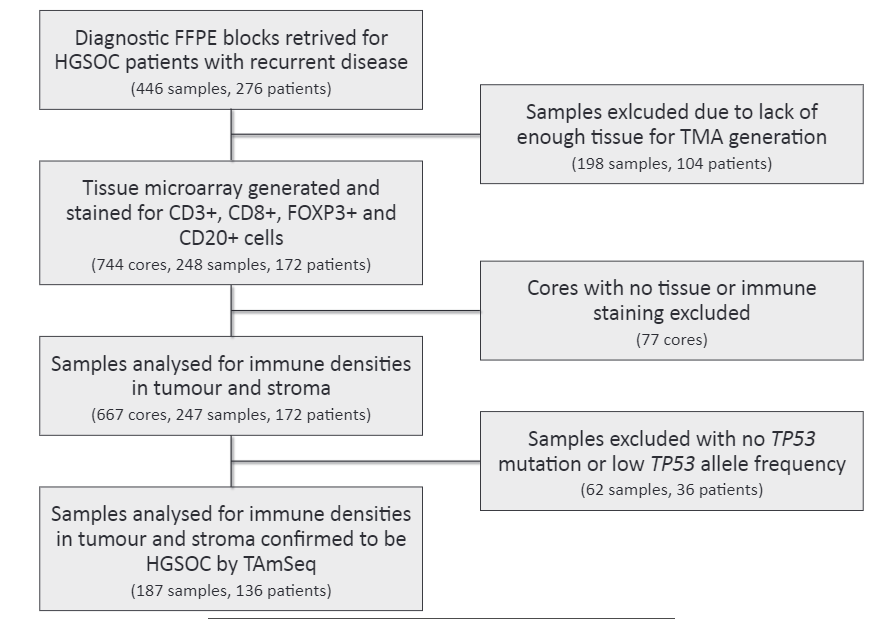
\includegraphics{Chapter4/figs/remark_britroc.png}
    \caption{REMARK diagram for the BriTROC cohort.}
    \label{fig:BriTROC_remark}
\end{figure}


\subsubsection{ICON7}
ICON7 was an international, phase 3, open-label, randomised trial undertaken at 263 centres in 11 countries across Europe, Canada, Australia and New Zealand. Eligible adult women with newly diagnosed ovarian cancer that was either high-risk early-stage disease (International Federation of Gynecology and Obstetrics [FIGO] stage I–IIa, grade 3 or clear cell histology) or more advanced disease (FIGO stage IIb–IV), with an Eastern Cooperative Oncology Group performance status of 0–2, were enrolled and randomly assigned in a 1:1 ratio to standard chemotherapy (six 3-weekly cycles of intravenous carboplatin [AUC 5 or 6] and paclitaxel 175 mg/m2 of body surface area) or the same chemotherapy regimen plus bevacizumab 7·5 mg per kg bodyweight intravenously every 3 weeks, given concurrently and continued with up to 12 further 3-weekly cycles of maintenance therapy. Randomisation was done by a minimisation algorithm stratified by FIGO stage, residual disease, interval between surgery and chemotherapy, and Gynecologic Cancer InterGroup group. The primary endpoint was progression-free survival; the study was also powered to detect a difference in overall survival. Analysis was by intention to treat. This trial is registered as an International Standard Randomised Controlled Trial, number ISRCTN91273375\cite{Perren2011Dec, BibEntry2020Jan}. Figure \ref{fig:icon_remark} is a REMARK diagram of samples analysed. TMA prepared by MRC.

ICON7 had cores sampled specifically from Epithelium and adjacent stroma, making it ideal for measurement of the microenvironment and measurement of both tumour and stroma in a single section which had been limited to a subset of the patients in previous cohorts.

\subsection{Immuno Metal Conjugation}
The protocol for IMC staining and imaging was carried out as described in Section \ref{sec:sarwah_staining}.

\subsection{Marker Panel}
The marker panel is specified in section \ref{table:imc_antibodies} and I worked with SAK to include Collagen in this panel for further investigation alongside the immune populations. 


\subsection{Staining and Imaging}
Staining and imaging of the BriTROC panel was carried out by SA-K. Staining and imaging of the ICON7 TMAs was carried out by Fatime Cosaj(FC) and Richard Grenfell(RG) accordingly.

\subsection{Image Analysis}
Python was used for data cleaning and Halo was used for the subsequent analysis of IMC data files. Structure analysis of signal in the collagen channel was carried out with Imagej and the GLCM, Orientationj and Directionality plugins. 


\section{Results}
Before analysing the interaction between these immune cells and these single populations on single tissue sections, I investigated the characteristics of the BriTROC and ICON7 cohorts are shown.

\subsection{BriTROC summary}
\subsection{ICON7 summary}

\subsection{IMC image analysis}
 In order to clean the data, I carried out hot-spot removal in python using a median filter with a 3x3 pixel area (see Code \ref{script:1}).
 I built a classifier in Halo to distinguish epithelial tissue from low density and high density collagen, specified by the intensity of the Collagen1 marker over small areas.
 I built other cell segmentation classifiers based on nuclear DNA1 and DNA2 marker stainings to segment nuclei and classify cells. 
 
 \begin{figure}
     \centering
     \includegraphics{IMC_example}
     \caption{Example of }
     \label{fig:IMC_example}
 \end{figure}

\subsection{Cell quantities and correlations}

The first investigation of this dataset was to investigate the correlations between immune populations to validate the results found in earlier chapters and to build up a picture of which features of the micro-environment are connected.

\begin{figure}
    \centering
    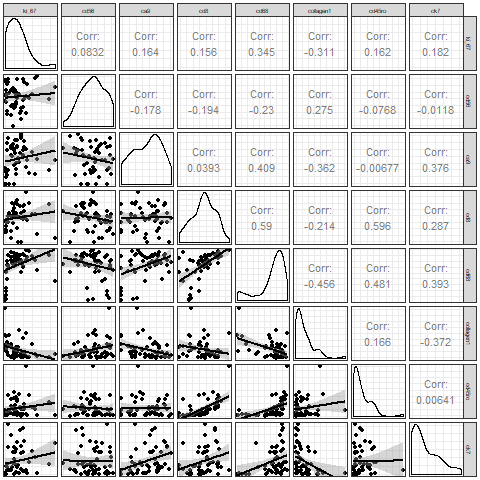
\includegraphics{Chapter4/figs/Britroc_cell_correlation2.png}
    \caption{Scatterplots of correlations between number of cells positive for each marker.}
    \label{fig:britroc_corr_scatt}
\end{figure}

\begin{figure}
    \centering
    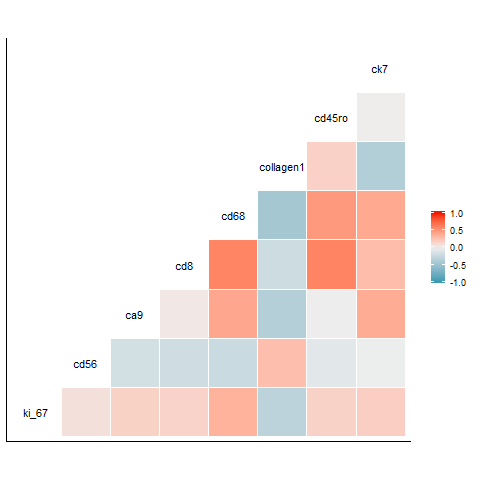
\includegraphics[width=\textwidth]{Chapter4/figs/Britroc_cell_correlation.png}
    \caption{Heatmap of correlations between number of cells positive for each marker.}
    \label{fig:britroc_corr_heat}
\end{figure}

Figures \ref{fig:britroc_corr_scatt} and \ref{fig:britroc_corr_heat} show the correlations between the number of CD8+, CD68+, CA9, CK7, Collagen1, CD45RO, CD56 and Ki-67+ cells. CD8, CD68 and CD45RO, the populations investigated in Chapter 1, show the strongest positive correlations. I also see the negative correlation we would expect between the number of Collagen and Cytokeratin positive cells as these cells are mutually exclusive and determine the majority of the structure of a tissue. Despite seeing a higher density of infiltrate in stromal regions in earlier chapters, we see a negative correlation between the number of collagen positive cells and the number of immune cells in these samples.

\subsection{Principal Component Analysis}
I carried out a similar PCA to Chapter 1 to analyse the key patterns across the. The first component was X.

\subsection{Comparing immune cell densities between epithelium, high density and low density collagen}

CD8
CD68
CD45RO
CD3

As shown here, dense collagen fibres exclude immune cells, loose collagen has a higher infiltration than epithelium.

\subsection{Collagen structure analysis}

\section{Discussion}
The ability to measure collagen deposition, patterns of immune infiltration and hypoxia simultaneously on one slide have led to a much more in depth and concrete results on the intersection between these.
Survival analysis showed that. 

